\section{Analysis 3: Do Frozen Models Benefit from Explicit Geometry?}

\paragraph{Motivation and hypotheses.} Idea 5 supplies explicit geometry (depth, segmentation, pose) for norm reasoning. Before training anything, we measure on frozen models what each kind of input contributes. \textbf{H1}: the answer text alone is not enough, and seeing the scene helps. \textbf{H2}: geometry maps add usable information beyond the RGB frames they are derived from.

\paragraph{Data and protocol.} From the released 200-item verified split of EgoNormia \citep{rezaei2025egonormia} we keep one item per source video and take the 60 with the sharpest frames, a choice based on image quality alone. Six frozen models answer each item from (i) the answer options only, (ii) the options plus five pre-action RGB frames, and (iii) those plus estimated depth (Depth Anything V2) and instance segmentation (YOLOv8n-seg) of the same frames. Each answer is a separate call with no shared context and counts only if action and justification are both correct. To see where geometry could matter, we also count how often the correct answers of all 1{,}853 items contain a term from a fixed spatial word list.

\begin{figure}[t]
\centering
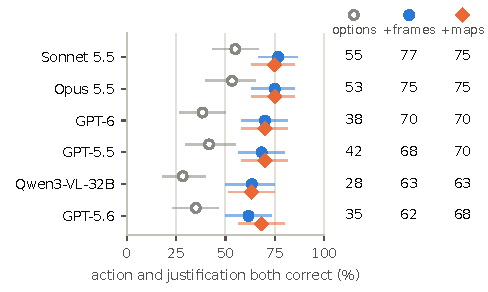
\includegraphics[width=\columnwidth]{analysis3_figure.pdf}
\caption{Joint accuracy of six frozen models on 60 items given the answer options only (grey), plus five RGB frames (blue), and plus depth and segmentation maps of those frames (orange). Lines are 95\% bootstrap intervals.}
\label{fig:a3}
\end{figure}

\paragraph{Results.} \emph{H1.} Text alone is not sufficient (Figure~\ref{fig:a3}): the options alone give 28--55\%, and adding frames raises accuracy by 27 points on average (95\% interval [16, 38]; each model $p\le0.03$, exact McNemar). \emph{H2.} Adding depth and segmentation then changes accuracy by $-2$ to $+7$ points, $+1.1$ on average [$-1.7$, $+4.2$]: across 360 model--item pairs, maps correct 17 answers and break 13, and no model's change is significant; the largest is GPT-5.6's gain of four answers ($+7$ points, $p=0.12$). The six items every model misses with frames stay wrong with maps. As a control, giving the same RGB grid three times instead of the maps does as well as the maps in all six models (256 vs.\ 253 of 360 answers correct; 249 with a single grid), and Qwen3-VL-32B scores 39/60 with another item's maps against 38 with its own. \emph{Where geometry could matter.} A spatial term appears in 24.6\% of correct answers, most often for Privacy (39.5\%) and Proxemics (33.4\%) and least for Cooperation (20.9\%); yet the 22 Proxemics items in our sample score 91 of 132 with or without maps.

\paragraph{Discussion of Analysis 3.} H1 holds and H2 does not. Multimodal input clearly adds value: frames add 27 points over the answer text. Geometry derived from those frames is neutral for a frozen model, neither helping nor hurting: repeating the frames does as well as adding the maps, and for Qwen another item's maps do as well as its own. Spatial content is also a minority signal, concentrated in Proxemics and Privacy, so any benefit should be looked for there. Limits: 60 items detect only large effects (about $\pm12$ points per accuracy), and sharp verified frames are a best case for the extractors. Most importantly, this does not test Idea 5 itself: these models were presumably never trained to read depth or segmentation maps beside RGB, so a frozen model cannot be expected to use them. Fine-tuning a model on such inputs is the real test, and it is our next experiment.
